\documentclass{article}
\usepackage{graphicx}
\usepackage[hyphens]{url}

\author{Ian Leinbach and Corin Rose}
\title{Inter-Planetary ID}

\begin{document}

\maketitle

\begin{center}
\textbf{Abstract} 
\end{center}

A universally agreed upon format for defining what data constitutes an ID would allow for interoperability between services. If this format is based on IPLD and represented as hash-linked data, we can leverage IPFS to store and share this information in a distributed way and let users maintain control of their data. By building off of amazing work done in distributed systems, we can create this format as a way of standardizing how a human exists on the Internet, in much the same way that, for example, Unicode standardized the way we represent arbitrarily complex symbols with data.  

\section{Introduction}
In IPID, an ID is simply a a folder of data hosted on IPFS which contains your data footprint--that is, all of the data you want to be associated with your public Internet identity, from contact info to published writing. We share this data by assigning an IPNS link to this data, which you can then give to people out of band (e.g. on a buisness card, or via a text). Then, you can update the IPFS folder pointed to by this name whenever you update your data, and anyone can always access this data with that same IPNS name. 

\section{Format}

\subsection{Data Serialization}

In an IPID folder, data should be future proof and self-describing in the sense of Multiformats.\footnote{\url{https://multiformats.io/}} Multiformats let us encode data in a consistent way, prefacing it with metadata about its content, and includes both a human-readable and binary representation. For example we can reference \texttt{foo.jpg}, a file stored on our own local machine over http on port 8000, by \texttt{/ip4/127.0.0.1/tcp/8000/http\-/foo.jpg}. This human-readable format can translated into a binary format with a lookup table for values of each protocol. Many types of content already do something like this, for example by declaring \texttt{<DOCTYPE! html>} in an HTML document. Any file in an IPID folder should make clear the way it is storing data.   

\subsection{Profile}

\begin{figure}[h]
  \centering
  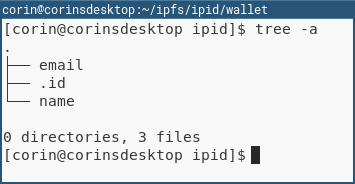
\includegraphics[width=.5\textwidth]{resources/basic_profile.png}
  \caption{A minimal profile.}
\end{figure}

We see in figure 1 an example of the most basic profile you can have. It consists of a "name," an "email," and a ".id" file. The name and email are both just plain text files with the name and email respectively. The name does not have to be a real name, it can be psuedononymous. The .id file contains the IPNS name of this profile, and acts as a flag that this folder is in fact an IPID folder. An ID needs to have at minimum a name and some kind of contact information, like email or phone. \par
Profiles can also include payment information in a "wallet" folder. For example, if you wish to post a Bitcoin recieving address to your profile, you can create "wallet/btc," a text file that contains your BTC address. See figure 2.

\begin{figure}[h]
  \centering
  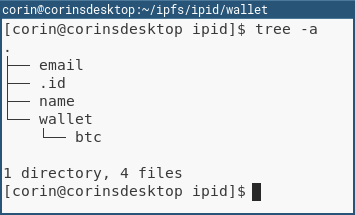
\includegraphics[width=.5\textwidth]{resources/basic_profile_wallet.png}
  \caption{A profile with a Bitcoin recieving address.}
\end{figure}

\subsection{Extensions}

We can easily define extensions to this format. A simple example is the wallet folder we saw above. Similarly, we could create a "blog" folder which contains a bunch of text files, each of which is a blog post. Then, anyone could write code that found this profile, looked through all of these posts, and formatted them nicely as a blog. \par
Organizations could also define their own extension paths to any depth. For example, if Vassar College wanted to integrate their data about me into my profile, they could create a "vassar" folder to add to the root folder, which would then include for example a student\_id file, and a transcript file, and so on. This third party format could also include subfolders. \\
Going further, a social media site or game could create a folder within one's data footprint to store data, leaving the user in control of their data. 

\section{IPFS}

We can easily host this folder on IPFS.

\begin{figure}[h]
  \centering
  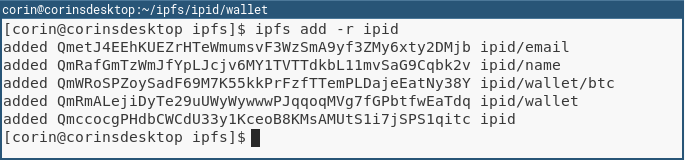
\includegraphics[width=.9\textwidth]{resources/profile_to_ipfs.png}
  \caption{Adding your IPID folder to IPFS.}
\end{figure}

Now, our IPID folder is can be accessed from anywhere at \\
  \texttt{/ipfs/QmccocgPHdbCWCdU33y1KceoB8KMsAMUtS1i7jSPS1qitc}. Exciting! 
This is not ideal, however, because now you must send a new IPFS link every time you update this information. Luckly, IPFS let's use name content! 

\begin{figure}[h]
  \hspace*{-2cm}
  \centering
  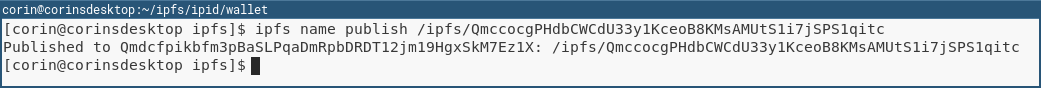
\includegraphics[width=.75\paperwidth]{resources/publish_profile.png}
  \caption{Publishing your IPID folder to your IPNS name.}
\end{figure}

Now, you can share \texttt{/ipns/Qmdcfpikbfm3pBaSLPqaDmRpbDRDT12jm19HgxSkM7Ez1X} with anyone and they will be able to find your up to date data over IPFS!



\section{Use Cases}

\subsection{Business Card}

One way to use this data footprint is to share it on a business card. This card can include a small QR code that encodes the IPNS path to the folder with your data. You can give out this business card to as many people as you'd like, and they will always be able to view your most up to date public data. 

\begin{figure}[h]
  \centering
  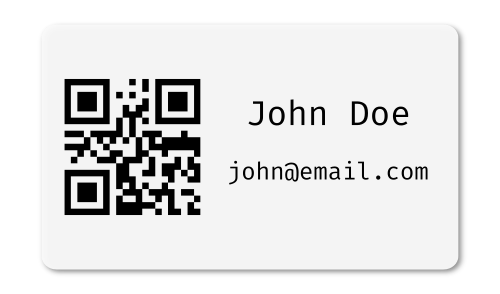
\includegraphics{resources/business_card.png}
  \caption{An example of a business card with a QR code that links to an ID over IPNS.}
\end{figure}

\section{Reference Implementation}

\subsection{Blog Extension}

\subsection{Profile Mirroring}

\section{Conclusion}

\end{document}
